%%CIShell: Cyberinfrastructure Shell (http://www.cishell.org)
%%
%%Draft Specification
%%Creation Date: June 12, 2006

\documentclass[a4]{article}
\usepackage{graphicx}

\title{CIShell: Cyberinfrastructure Shell\\A Novel Algorithm Integration
Framework\thanks{Developed at Indiana University's Cyberinfrastructure for
Network Science Center}\\
\textbf{DRAFT}
} 
\author{Bruce Herr (bh2@bh2.net) 
\and Weixia (Bonnie) Huang (huangb@indiana.edu)
\and Shashikant Penumarthy (sprao@indiana.edu)
\and Katy B\"{o}rner (katy@indiana.edu)
}

\begin{document}

\maketitle{}
\tableofcontents{}

\newpage{}

\section{Introduction}

\subsection{The Problem}

In the scientific world, we have a problem: We are duplicating our efforts.
Toolkits with much the same functionality are worked on for years and force
algorithm developers to write just for their framework to work. Many algorithms
are implemented multiple times due to not knowing about each other, idealogical
reasons, or incompatible toolkits. Algorithms are accessed and run in many,
many ways. Some are stuffed in a directory on a remote machine and must be
run manually on the command line and require varying file formats for
input/output. Some are only available in certain toolkits, and others require
programming to their api just to run them.

So, what is wrong with having multiple implementations of algorithms and 
incompatible toolkits? Its a waste of time, of which we have little of. If 
there were an open framework for integrating algorithms, we could save much 
time and effort. This framework would not be a one stop shop for all your 
toolkit and algorithm needs though. We need competition, but on a more level 
(and sane) playing field that encourages innovation and cooperation. If we were 
to define how to integrate algorithms, then toolkit developers would be 
encouraged to make novel clients on top of the integration framework. Algorithm 
developers would vie with one another solely on the merit of their 
implementation and not have to worry about any other issues such as 
distribution, user interfaces, or toolkits. We could now have algorithm 
developers concentrating on algorithms, toolkit developers concentrating on 
toolkits, and scientists finally concentrating on doing science. In the end, 
this will speed scientific progress and best use humanity's global brain.

\subsection{A Solution}

CIShell: Cyberinfrastructure Shell is an open source, community-driven 
framework for integration of diverse algorithms, data, and computing power. It 
provides a standard framework for algorithm developers to quickly get their 
algorithm into the system and a base upon which novel clients to the algorithms 
can be built on.

\footnotetext[1]{http://www.osgi.org}

In the spirit of not duplicating effort, CIShell is built upon the 
OSGi\footnotemark[1] (Open Services Gateway Initiative) Framework. OSGi is a 
standardized, component oriented, computing environment for networked services.
Founded in 1999, it has had much success in the commercial business world from
high-end servers to embedded mobile devices. In the open source realm, it is
finding more adoption, especially since Eclipse has moved its plugin model to
OSGi R4 starting with version 3.0 of eclipse. OSGi is a powerful framework that
will enable us to have a truly capable system.

CIShell is all about integrating algorithms. The base framework defines a 
standard for creating, accessing and running algorithms, services that the 
algorithms can use, and separate services that toolkit developers can use to 
create clients on top of the framework.

For the purposes of this framework, we have made some assumptions. First, we
consider algorithms to be black boxes. We don't know what goes on when we call
on the algorithm to execute, we only assume that it takes in some data and
spits out some data. What happens in between, we stay out of. Second, we have
not addressed doing coupled displays with brushing and linking, though we are
confident that the CIShell Framework should be able to accomodate it in the
future. Finally, for the purposes of remote execution we do not address
visualizations in this context. For our purposes we have assumed that remote
execution will not be used for visualization, though ways to do this will be
explored in the future.

\section{The Framework}
\label{TheFramework}

The CIShell Framework defines an algorithm service, the standard services that 
algorithms can use, and separate services that client applications can use. In 
this section we will define these services and explain how they will be used 
together in the framework. In section \ref{TheClients}, we will take you 
through how several prototypical clients would work.

A basic understanding of OSGi and Java is assumed here. If you are not familiar 
with its terminology, please go to http://www.osgi.org/osgi\_technology/ for a 
brief introduction to the technology.

\subsection{Algorithm Definition}

Algorithms in this system are packaged as standard OSGi bundles and integrated 
into the system as services. There can be multiple algorithm services 
registered from one bundle, but for each algorithm there will be only one 
associated OSGi service. To be a service in the OSGi framework, a bundle must 
provide three things: a Dictionary of key/value pairs (properties of the 
service), one or more interfaces, and an instantiated implementation of the 
interface(s). In the following sections we will describe what properties are
needed and define the service interfaces that must be implemented.

\subsubsection{Standard Algorithm Properties}

To have an algorithm integrated into the system, algorithm developers must 
provide the proper meta-data to describe it. These properties are very 
important, because based on the properties, we can query the ServiceRegistry 
and do things like finding algorithms we need, finding where we need to put the 
algorithms in a menu, and figuring out what meta-data should be shown to the 
user. Below we will define an initial list of possible properties and how they 
would be used in the system.

\begin{itemize}
\item {\bf menu\_location=``menu/location/path/additions''} -- Where an algorithm
should go in the menu
\item {\bf label=``My Algorithm Label''} -- The label to use
\item {\bf in\_data=``java.class.name or file:type or Null or file-ext:ext,
\ldots''} -- What type of data it will take in
\item {\bf out\_data=``java.class.name or file:type or Null or file-ext:ext,
\ldots''} -- What type of data it will create when run
\item {\bf remoteable=``true or false''} -- if the algorithm can be run on a
remote server
\item {\bf remote=``http://remoteserver.com:1000''} -- if an algorithm is a remote algorithm,
where it is being hosted at
\item {\bf conversion=``lossy or lossless''} -- if an algorithm is a converter,
then whether the conversion is lossless or lossy. Otherwise it should not be set.
\item {\bf complexity=``O(complexity)''} -- An estimate of the big-O complexity
of the algorithm
\item {\bf description=``Algorithm Description''} -- A short description of the
algorithm
\item {\bf citation=``citation text for citing''} -- A citation to use when
citing this algorithm
\item {\bf citation\_url=``http://scholar.com/a.pdf''} -- A URL to the cited paper
\item {\bf implementor=``Implementor's Name, \ldots''} -- The name(s) of the implementor(s)
of the algorithm\item 
\item {\bf documentation\_url=``http://my\_documentation.com''} -- An URL where
the documentation for the algorithm is
\end{itemize}

\subsubsection{Algorithm Interfaces}

An algorithm service consists of two main classes: the AlgorithmFactory and the 
Algorithm. An AlgorithmFactory has two main tasks. First, an AlgorithmFactory 
provides the parameters that are needed to create an Algorithm. Second, when 
the client gives it a data model, a dictionary with the parameter values, and a 
CIShellContext, the AlgorithmFactory will use this data to create an Algorithm.

\begin{verbatim}
public interface AlgorithmFactory {
    public MetaTypeProvider createParameters();
    public Algorithm newInstance(DataModel[] dm, 
                                 MetaTypeProvider parameters, 
                                 CIShellContext context);
}
\end{verbatim}

The basic Algorithm interface is very simple. It only has an execute method. 
This is because the algorithm factory already gave it all the information it 
needs to run (data, parameters, and context). Now all that needs to be done is 
crank the execute method and the algorithm will run and return a set of zero or 
more DataModels representing the data it created.

\begin{verbatim}
public interface Algorithm {
   public DataModel[] execute(); 
}
\end{verbatim}

The AlgorithmFactory and the Algorithm can extend more interfaces if it wishes 
to provide more service. An AlgorithmFactory can implement DataModelValidator 
if it wishes to validate the DataModel more than what is provided in the 
algorithm properties file. An example would be, if an algorithm worked on a 
Matrix, but required it to be a symetric matrix. If an Algorithm can be stopped 
midstream, it can implement the Stoppable interface to allow this. 
Finally, if an Algorithm can report on the progress of its algorithm, it can 
implement ProgressTrackable.

\begin{verbatim}
public interface DataModelValidator {
    public boolean supports(DataModel[] dm);
    public String unsupportedReason(DataModel[] dm);
}

public interface Stoppable {
    public void stop();
    public boolean isStopped();
}

public interface ProgressTrackable {
    public int getProgress();
}
\end{verbatim}

There are three more interfaces that an algorithm service writer must consider:
DataModel, CIShellContext, and MetaTypeProvider. The DataModel holds both the actual data
(represented as a Java Object) and its meta-data. The CIShellContext is used by
algorithms to gain access to standard services provided by the CIShell Framework
such as logging, preferences, and data conversion services. These standard
services will be described in section \ref{AlgorithmServices}. Finally,
MetaTypeProvider is documented in the OSGi standard as part of the metatype
service\footnotemark[2]. It is basically a way to describe what parameters will be needed. 

\footnotetext[2]{This is well documented in section 105 of the OSGi R4 Reference
Compendium located in the technology section of osgi.org}

\begin{verbatim}
public interface DataModel {
    public Object getProperty(String key);
    public String[] getPropertyKeys();
    public void setProperty(String key, Object value);
    
    public Dictionary getProperties();
    public Object getData();
}

public interface CIShellContext {
    public Object getService(String service);
}
\end{verbatim}

\subsection{Algorithm Services}
\label{AlgorithmServices}

The CIShell Framework provides several standard services that an algorithm can
gain access to. The four first standard services are the PreferencesService,
LogService, ConversionService, and GUIBuilderService. An algorithm gains access
to these services through the CIShellContext. One should note here, that you
could actually get these services through the ServiceRegistry, but by getting
them through the CIShellContext, it allows clients to return proxied services
that could pipe output to remote clients (this will be explained more in section
\ref{RemoteServer}).

The PreferencesService allows an algorithm to save configuration information
between sessions. This service is provided by the standard OSGi
framework\footnotemark[3].
\footnotetext[3]{section 106 of the OSGi R4 Reference
Compendium} 

\begin{verbatim}
public interface PreferencesService {
    public Preferences getSystemPreferences();
    public Preferences getUserPreferences(String name);
    public String[] getUsers();
}
\end{verbatim}

The LogService provides a standard logging mechanism for algorithms to use. This
service is also provided by the standard OSGi framework\footnotemark[4]
\footnotetext[4]{section 101 of the OSGi R4 Reference
Compendium}

\begin{verbatim}
public interface LogService {
    public void log(int level, String message);
    public void log(int level, String message, Throwable exception);
    public void log(ServiceReference reference, int level, String message);
    public void log(ServiceReference reference, int level, String message,
                    Throwable exception);
}
\end{verbatim}

The ConversionService is a CIShell defined service that is actually a thin 
client to the algorithm services. It searches for AlgorithmFactory services 
that have the conversion property set and creates a graph so that when an 
algorithm (or whoever accesses the service) asks for a way to convert from 
DataModel A to DataModel C, it will search its service graph for the optimal 
sequence of converters to use to convert from A to C. For clients, this 
conversion service can be used to do automatic conversions so a user will never 
have to convert data types again. \textit{Note that the interface for this 
service is not finalized.}

\begin{verbatim}
public interface ConversionService {
    public AlgorithmFactory converterFor(int max_hops, String max_complexity,
                                         String in_format, String out_format);
}
\end{verbatim}

Finally, the GUIBuilderService is a CIShell defined service that allows
algorithms to display simple GUIs and pop-ups to the user when needed. The GUI
is built from a given MetaTypeProvider as defined in the OSGi specification.
This GUI Builder simplifies the GUI creation process for algorithms. An
algorithm need only describe what values are needed and in what range and the
GUI builder will take care of translating that into a GUI for data input. Also,
since the GUIBuilderService is a part of the standard CIShell services, it can
be used when running remotely to display GUIs on the connected machine. 
\textit{Note that the interfaces for this service is not finalized.}

\begin{verbatim}
public interface GUIBuilderService {
    public GUI createGUI(MetaTypeProvider parameters);
    public GUI createPopUp(String popupType);
}

public interface GUI {
    public void open();
    public void close();
    public void setSelectionListener(SelectionListener listener);
}

public interface SelectionListener {
    public boolean hitOk(Dictionary valuesEntered);
}
\end{verbatim}

\subsection{Client Services}

The CIShell Framework also defines several services that clients to the 
algorithms can use in addition to the standard algorithm services. These 
services could also be used by the algorithms, but it is strongly discouraged 
to simplify both the algorithm and client writers' jobs. The two first standard 
client services are the SchedulerService and the ModelManagementService.

The SchedulerService allows the client to schedule algorithms to be run either
immediately or at a certain time. The service will allow a user-defined number
of algorithms to be run at the same time. \textit{Note that the interfaces for
this service is not finalized.} 

\begin{verbatim}
public interface Scheduler {
    public void runNow(Algorithm algorithm);
    public void schedule(Algorithm algorithm);
    public void schedule(Algorithm algorithm, Calendar time);
    public boolean unschedule(Algorithm algorithm);
    public boolean reschedule(Algorithm algorithm, Calendar newTime);
    public void addSchedulerListener(SchedulerListener listener);
    public void removeSchedulerListener(SchedulerListener listener);
    public boolean isRunning();
    public boolean isEmpty();
}

public interface SchedulerListener {
    public void algorithmMovedToRunningQueue(Algorithm algorithm, int index);
    public void algorithmScheduled(Algorithm algorithm, Calendar time, int index);
    public void algorithmScheduled(Algorithm algorithm, Calendar time);
    public void algorithmStarted(Algorithm algorithm);
    public void algorithmFinished(Algorithm algorithm, DataModel[] createdDM);
    public void algorithmError(Algorithm algorithm, Exception error);
}
\end{verbatim}

The ModelManagerService allows the client to manage models that are loaded into
memory. \textit{Note that the interfaces for this service is not finalized.} 

\begin{verbatim}
public interface ModelManager {
    public void addModel(DataModel model);
    public void removeModel(DataModel model);
    public Set getSelectedModels();
    public void setSelectedModels(Set models);
    public Set getModels();
}
\end{verbatim}

\subsection{Putting it All Together}

In this section we will try to give you several views to help see how the 
CIShell Framework fits together. In Figure \ref{ClassInteractionDiagram}, you 
can see how the different objects interact with one another. Figure 
\ref{serviceDiagram} shows how the services interact in the system. Figure 
\ref{algorithmViewWorkflow} shows the three workflow scenarios an algorithm 
writer has to deal with. And finally, Figure \ref{clientViewWorkflow} shows 
what a typical client's workflow would be like.

\begin{figure}
\centering
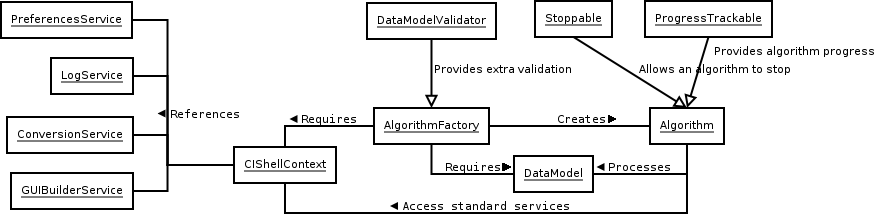
\includegraphics[width=120mm]{graphics/classDiagram.png}
\caption{Class Interaction Diagram}
\label{ClassInteractionDiagram}
\end{figure}

\begin{figure}
\centering
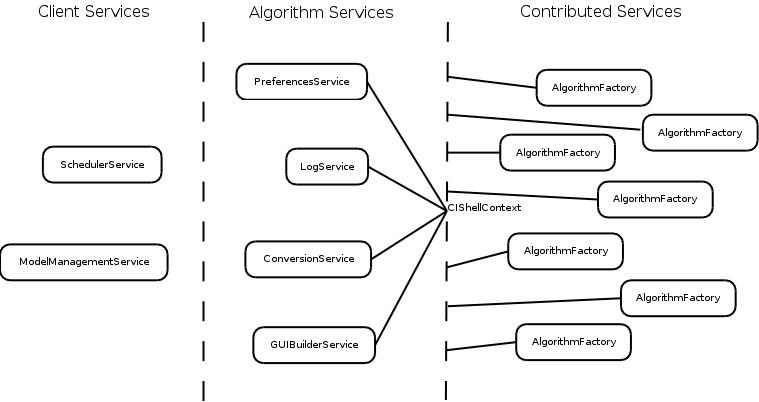
\includegraphics[width=120mm]{graphics/serviceDiagram.png}
\caption{Service Diagram}
\label{serviceDiagram} 
\end{figure}

\begin{figure}
\centering
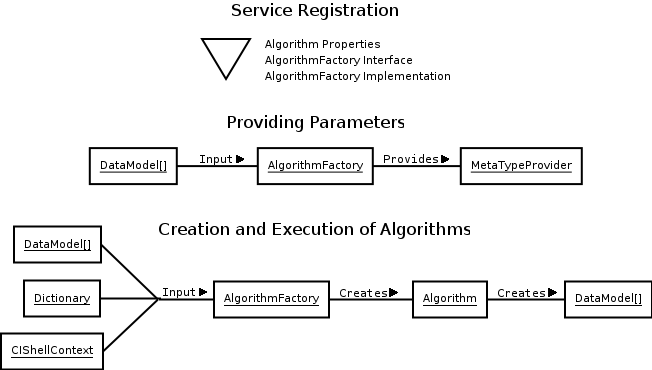
\includegraphics[width=120mm]{graphics/algorithmViewWorkflow.png}
\caption{Workflows from an Algorithm's Perspective}
\label{algorithmViewWorkflow} 
\end{figure}

\begin{figure}
\centering
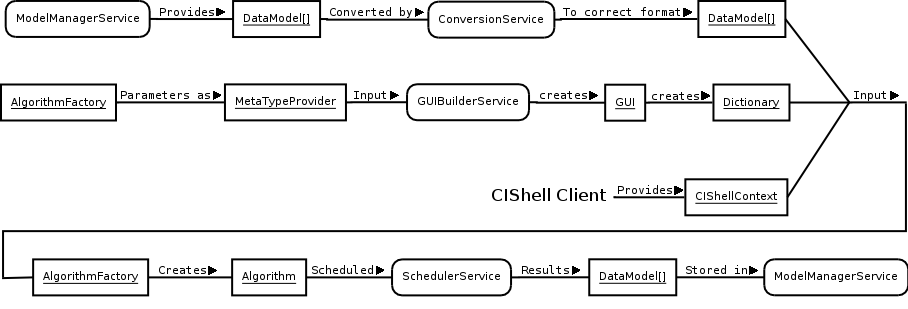
\includegraphics[width=120mm]{graphics/clientViewWorkflow.png}
\caption{Typical Workflow from a Client's Perspective}
\label{clientViewWorkflow} 
\end{figure}

\section{Some Prototypical Clients}
\label{TheClients}

In section \ref{TheFramework} we defined the CIShell Framework. Now we will 
explain how some typical clients could use the framework. There is power in 
providing the algorithms uniformly in that now we can support any way that the 
user wishes to work. For example, the framework can be used as a typical GUI 
application, as a remote service, as a scripting engine, and most excitingly as 
a peer-to-peer client for sharing data, algorithms, and computing power!

\subsection{Standard GUI}

\begin{figure}
\centering
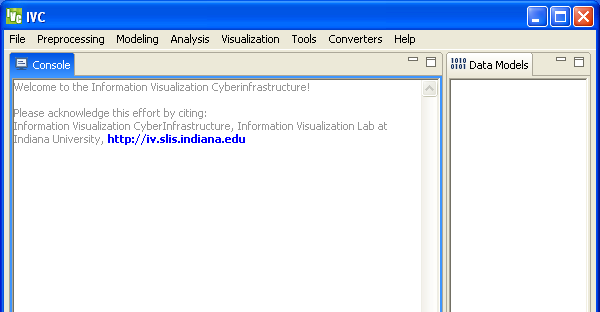
\includegraphics[width=120mm]{graphics/guiApplication.png}
\caption{Typical GUI client application, IVC}
\label{guiApplication}
\end{figure}

\footnotetext[5]{http://sourceforge.net/projects/ivc}
\footnotetext[6]{http://nwb.slis.indiana.edu}

The CIShell Framework should work beautifully with a GUI client. The previous 
iterations of this project were all GUI based, so by far this is the most 
supported. For making a client like the Information Visualization 
Cyberinfrastructure Tool\footnotemark[5] (shown in figure \ref{guiApplication}) 
or the Network Workbench Tool\footnotemark[6], both developed at IU, there 
would be several steps. First, after the system has been brought up, the GUI 
client would query the service registry to find all of the AlgorithmFactory 
services and based upon their meta-data, would create menu items that when 
clicked would pull out the AlgorithmFactory and follow the workflow from figure 
\ref{clientViewWorkflow}.

\subsection{Web Front-End}

A web front-end could be done exactly like the GUI client, only using web
technologies to produce the UI in a web-browser.

\subsection{Remote Server}
\label{RemoteServer}

A remote server could be created by setting up services on both ends (local and 
remote) that would create proxies for the algorithms and services offered by 
CIShell. The local client would then just see new algorithms and would 
(basically) have to do nothing differently, since all of the complexity is 
behind the proxies. When the local client asks for an Algorithm from the 
AlgorithmFactory it returns a proxied Algorithm, and when executed, it runs on 
the remote server. On the remote server, when the local client requests an 
AlgorithmFactory to return an Algorithm, instead of giving the AlgorithmFactory 
the CIShellContext for the remote server, it would pass it a context that held 
proxied services corresponding to the standard CIShell services on the local 
client. Many design decisions were made with this scenario in mind.

\subsection{Peer-to-peer sharing}

Peer-to-peer sharing would be similar to a remote server. The major difference
would be that the client machine would share its algorithms and services with
the server machine. Then each peer would allow other peers to connect to it in
the same way to build a peer-to-peer network. This is an exciting possibility
that we hope to look into further in the future.

\subsection{Scripting Engine}

A scripting engine would allow a script writer to go through much of the
workflow described in figure \ref{clientViewWorkflow} programmatically using the
host scripting language. Most commands provided would then just be analogs to
the workflow, with perhaps some changes to make it easier for script writing. A
GUI client could also output these scripts as logs of what a user did for
playback at a later time to confirm results with colleagues.

\subsection{Workflow-Engine}

A workflow engine would act mainly like a scripting engine in that it creates
its itenerary of things to do ahead of time and runs it later. However, it could
also use aspects of a GUI client and utilize remote servers.

\end{document}
